\documentclass[crop,tikz,convert={outext=.svg,command=\unexpanded{pdf2svg \infile\space\outfile}},multi=false]{standalone}

\usepackage{amsmath}
\usepackage{amssymb}
\usepackage{mathtools}
\usepackage{fullpage}
\usepackage[T1]{fontenc}
\usepackage{lmodern}
\usepackage{tikz}
\usetikzlibrary{calc,intersections,through,backgrounds}
\usetikzlibrary{bayesnet}
\usepackage{tikzscale}
\usepackage{tkz-euclide}
\usepackage{tcolorbox}
\tcbuselibrary{skins,breakable}
% pgfplots
\usepackage{pgfplots}
\pgfplotsset{compat=1.8}
% For entities in text
\newcommand{\entity}[1]{\texttt{#1}}
% For entities in pgfplots
\newcommand{\entpgf}[1]{\texttt{#1}}

\begin{document}
	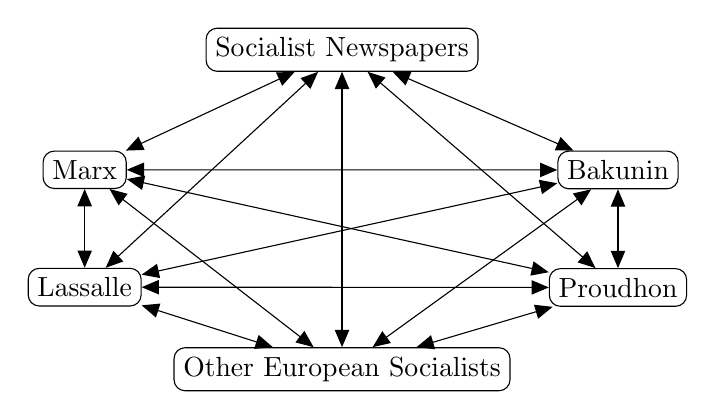
\begin{tikzpicture} %
		% Center
		\node[draw, rounded corners] (News) {Socialist Newspapers} ;
		\node[draw, below left=of News, rounded corners] (Marx) {Marx} ; %
		\node[draw, below right=of News, minimum width=8.5mm, rounded corners] (Bakunin) {Bakunin} ; %
		% Left
		\node[draw, below=of Marx, rounded corners] (Lassalle) {Lassalle} ;
		\node[draw, below=of Bakunin, rounded corners] (Proudhon) {Proudhon} ;
		%\node[right=of atp1] (atp2) {$\ldots$} ;
		% Fake nodes for getting the spacing right
		\node[below=of News] (Blank1) {} ;
		\node[below=of Blank1] (Blank2) {} ;
		\node[draw, below=of Blank2, rounded corners] (EuroSoc) {Other European Socialists} ;
		\edge [<->] {Marx} {Bakunin} ;
		\edge [<->] {Marx} {Lassalle} ;
		\edge [<->] {Marx} {Proudhon} ;
		\edge [<->] {Marx} {News} ;
		\edge [<->] {Marx} {EuroSoc} ;
		\edge [<->] {Bakunin} {Lassalle} ;
		\edge [<->] {Bakunin} {Proudhon} ;
		\edge [<->] {Bakunin} {News} ;
		\edge [<->] {Bakunin} {EuroSoc} ;
		\edge [<->] {Lassalle} {Proudhon} ;
		\edge [<->] {Lassalle} {News} ;
		\edge [<->] {Lassalle} {EuroSoc} ;
		\edge [<->] {Proudhon} {News} ;
		\edge [<->] {Proudhon} {EuroSoc} ;
		\edge [<->] {News} {EuroSoc} ;
	\end{tikzpicture}
\end{document}
